%%%%%%%%%%%%%%%%%%%%%%%%%%%%%%%%%%%%%%%%%%%%%%%%%%%%%%%%%%%%%%%%%%%%%%%%%
 
\begin{figure}[p]
\begin{center}
\begin{tabular}{cc}
  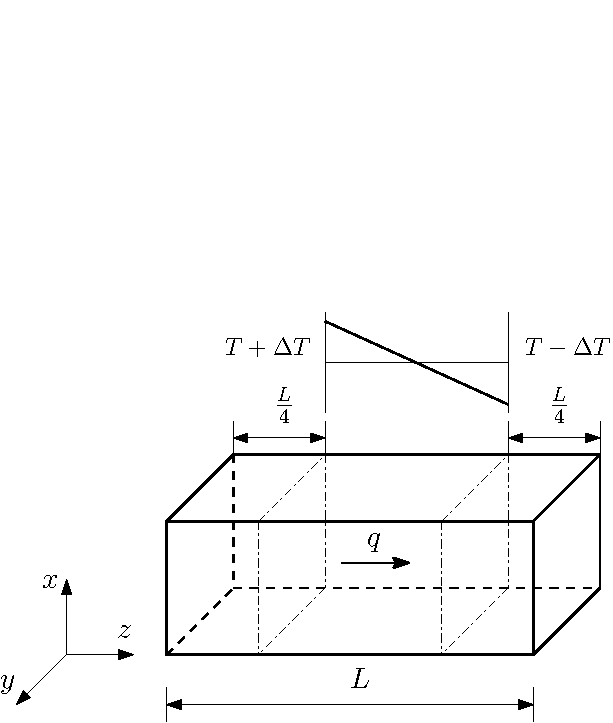
\includegraphics[width=0.48\textwidth]{./Figures/schematic}
  &
  \hspace{3mm}
  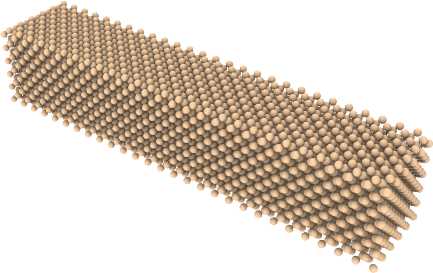
\includegraphics[width=0.40\textwidth]{./Figures/Sibar_05}
  \\ (a) & (b)
  \end{tabular}
\caption{(a) Schematic illustration of the set-up for evaluating thermal conductivity of Si using NEMD. (b) 
Arrangement of Si atoms prior to the application of thermal gradient.}
\label{fig:setup}
\end{center}
\end{figure}

\clearpage

%%%%%%%%%%%%%%%%%%%%%%%%%%%%%%%%%%%%%%%%%%%%%%%%%%%%%%%%%%%%%%%%%%%%%%%%%

\begin{figure}[p]
 \begin{center}
  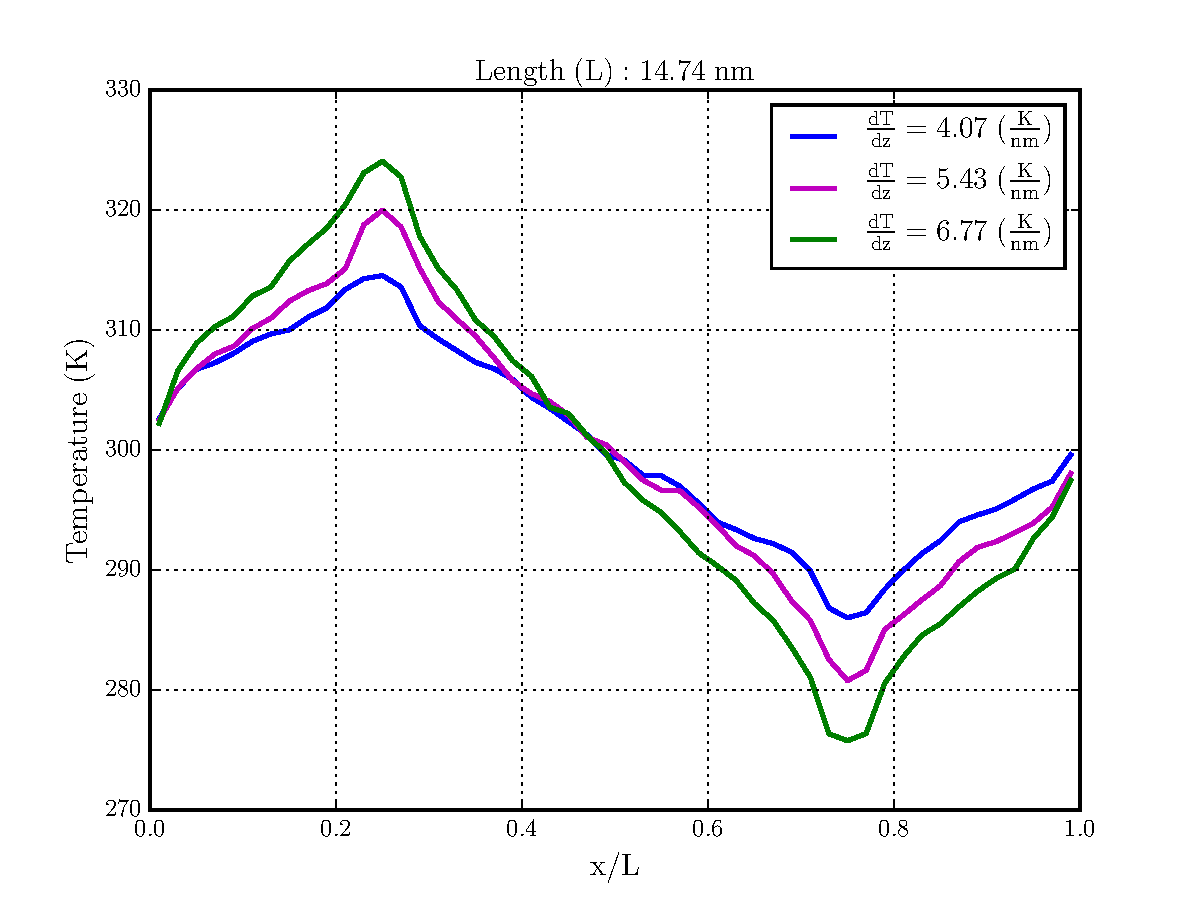
\includegraphics[width=0.70\textwidth]{./Figures/temp_plot}
\caption{Temperature distribution along a Si bar of length 14.74~nm for different scenarios of applied 
thermal gradient.}
\label{fig:kapitza}
\end{center}
\end{figure}


\clearpage

%%%%%%%%%%%%%%%%%%%%%%%%%%%%%%%%%%%%%%%%%%%%%%%%%%%%%%%%%%%%%%%%%%%%%%%%%

\begin{figure}[p]
\begin{center}
\begin{tabular}{cc}
  \hspace{-12mm}
  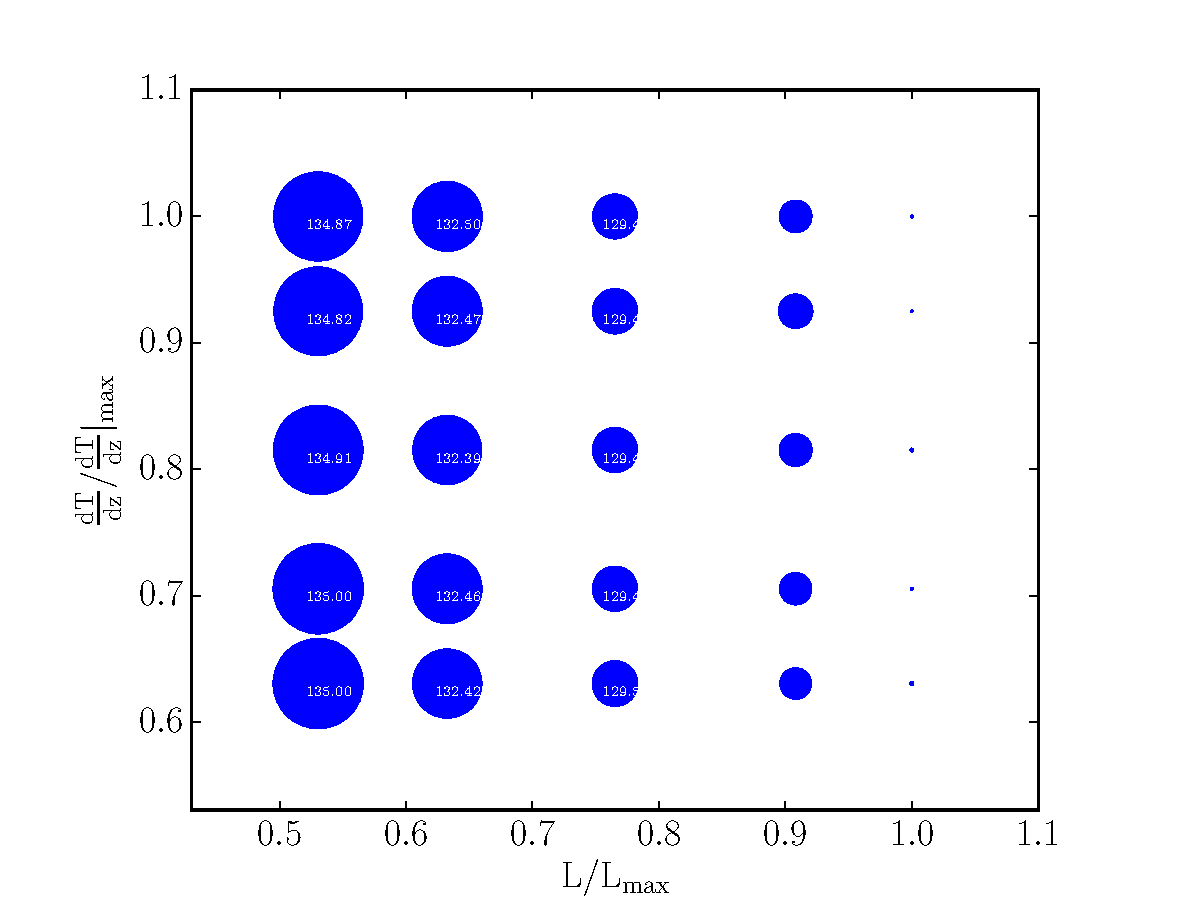
\includegraphics[width=0.60\textwidth]{./Figures/realz_quad300K}
  &
  \hspace{-9mm}
  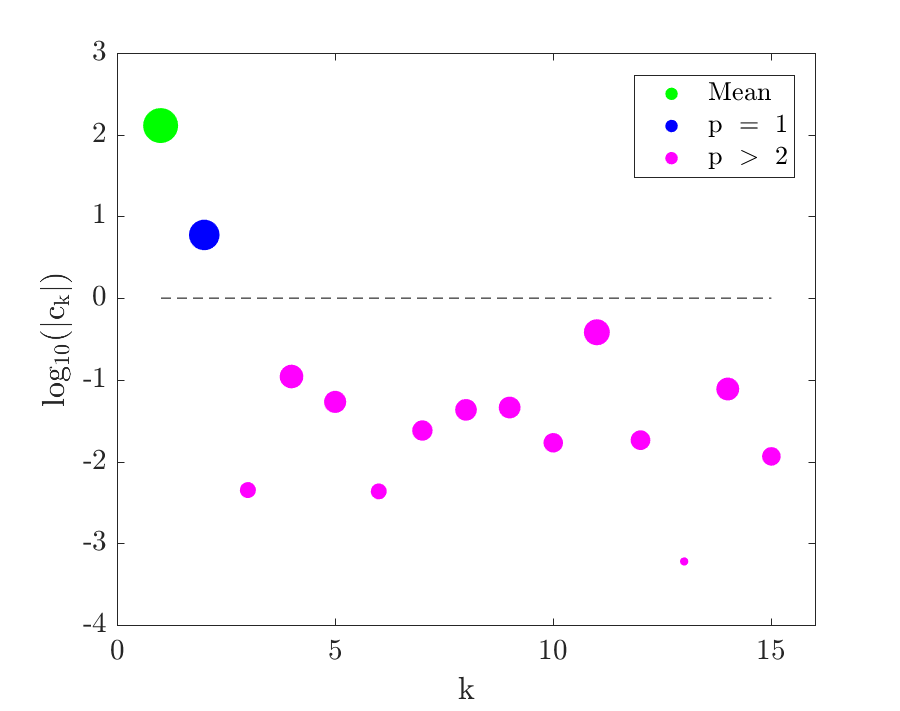
\includegraphics[width=0.56\textwidth]{./Figures/PCspectrum_300}
  \\ (a) & (b)
  \end{tabular}
\caption{(a) Realizations of discrepancy in bulk thermal conductivity at the Gauss-Legendre quadrature notes are
depicted using circles. The size of the circle in each case is proportional to the discrepancy estimate, also provided
 in cases where it is observed to be relatively large. (b) Spectrum of PC coefficients is depicted using circles of
 varying sizes, proportional to the log value of their magnitude. The computations were performed at 300 K.}
\label{fig:rs1}
\end{center}
\end{figure}

\clearpage

%%%%%%%%%%%%%%%%%%%%%%%%%%%%%%%%%%%%%%%%%%%%%%%%%%%%%%%%%%%%%%%%%%%%%%%%%

\begin{figure}[p]
\begin{center}
\begin{tabular}{cc}
 \hspace{-10mm}
  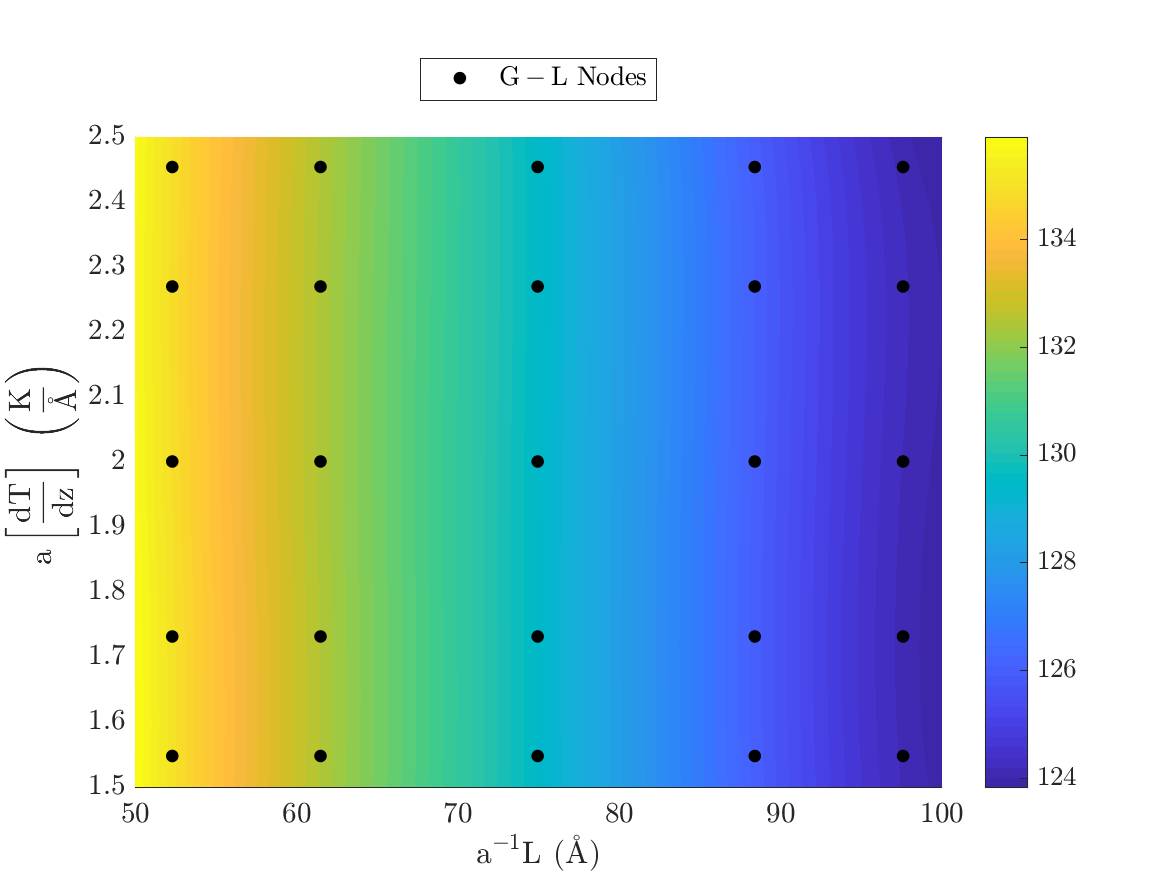
\includegraphics[width=0.55\textwidth]{./Figures/err2D_300}
  &
  %\hspace{-9mm}
  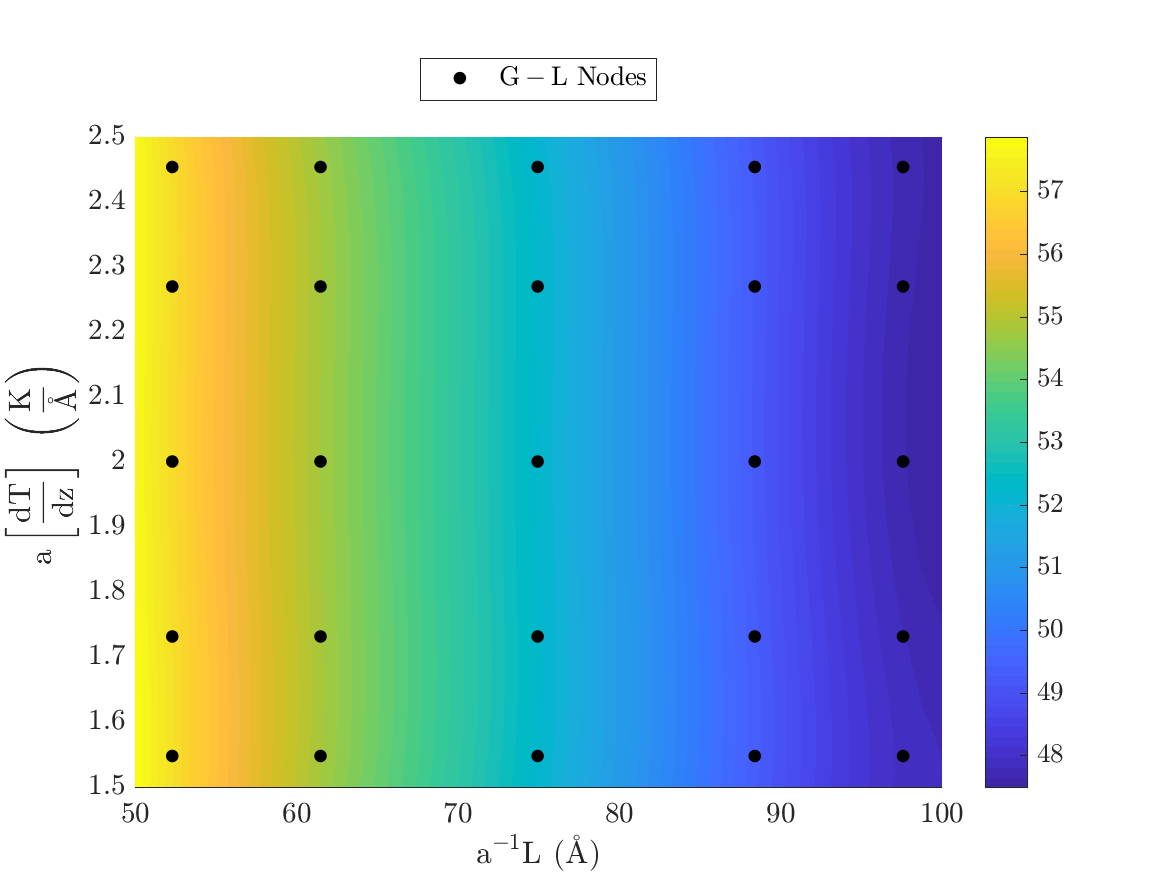
\includegraphics[width=0.55\textwidth]{./Figures/err2D_500}
  \\ (a) & (b)
  \end{tabular}
  \\ \vspace{1mm}
  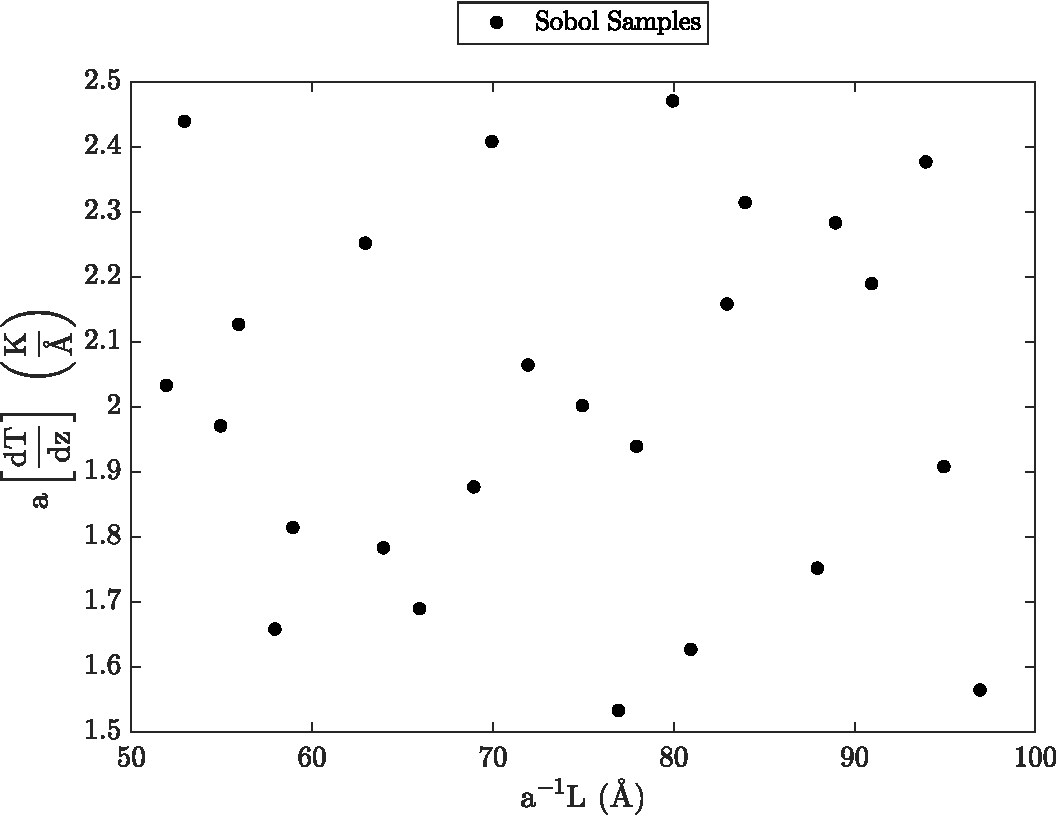
\includegraphics[width=0.50\textwidth]{./Figures/err2D_s}
  \\ (c)
\caption{Response surface of the discrepancy in bulk thermal conductivity at (a) $T$ = 300~K and
 (b) $T$ = 500~K. Gauss-Legendre quadrature nodes are highlighted in both cases. (c) Sobol samples
 in the 2D domain used for verifying the accuracy of the response surfaces.}
\label{fig:rs2}
\end{center}
\end{figure}

\clearpage

%%%%%%%%%%%%%%%%%%%%%%%%%%%%%%%%%%%%%%%%%%%%%%%%%%%%%%%%%%%%%%%%%%%%%%%%%

\begin{figure}[p]
\begin{center}
\begin{tabular}{cc}
 \hspace{-10mm}
  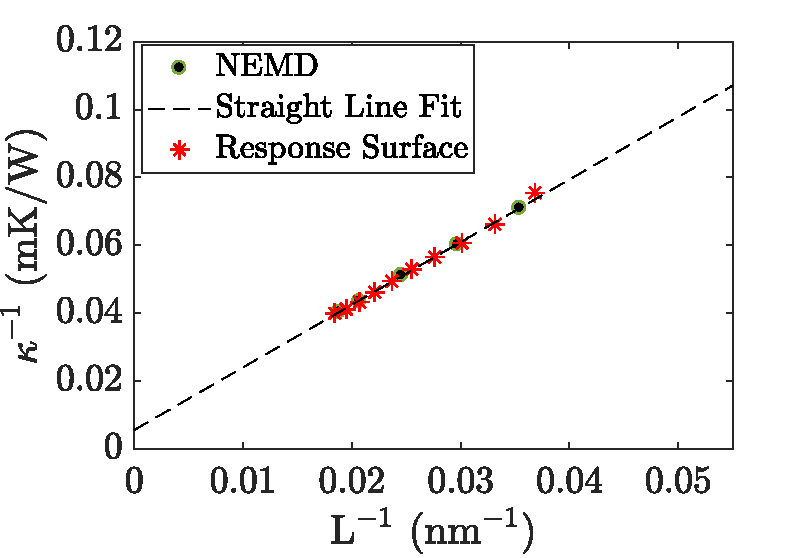
\includegraphics[width=0.50\textwidth]{./Figures/kinv_300}
  &
  %\hspace{-9mm}
  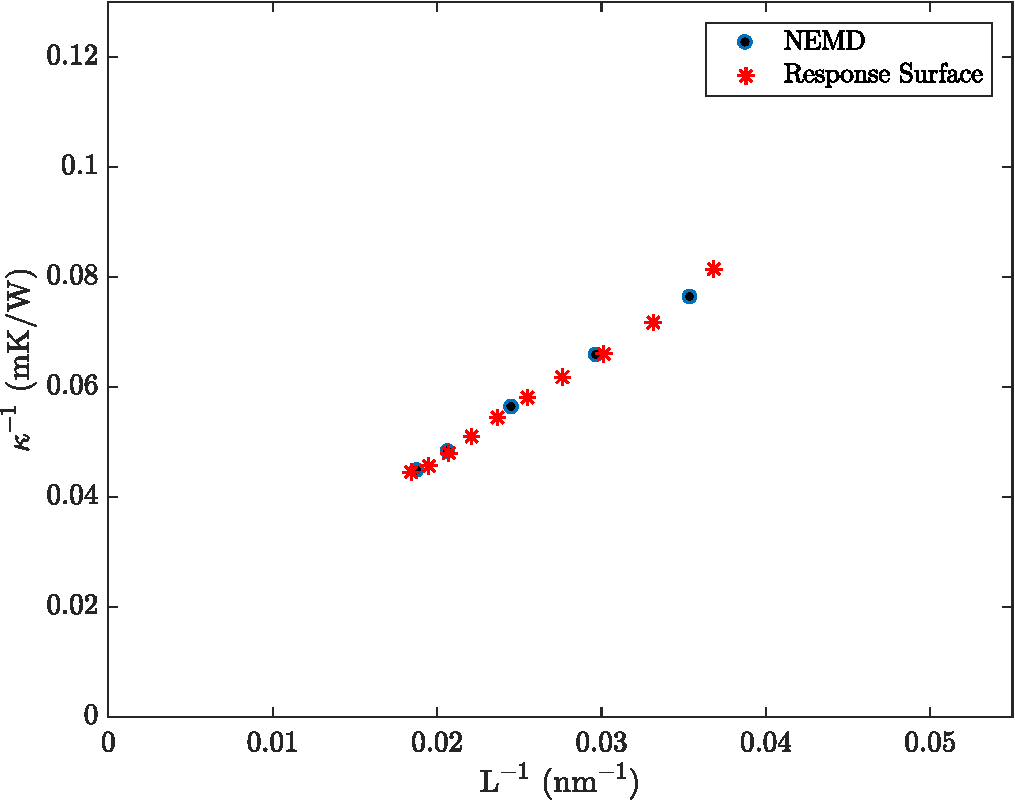
\includegraphics[width=0.50\textwidth]{./Figures/kinv_500}
  \\ (a) & (b)
  \end{tabular}
 \caption{Inverse of the bulk thermal conductivity estimates are plotted against the inverse of Si bar length
 using predictions from NEMD as well as estimates from the response surface at (a)  $T$ = 300~K and 
 (b) $T$ = 500~K.}
\label{fig:rs3}
\end{center}
\end{figure}

\clearpage

%%%%%%%%%%%%%%%%%%%%%%%%%%%%%%%%%%%%%%%%%%%%%%%%%%%%%%%%%%%%%%%%%%%%%%%%%
 
\begin{figure}[p]
\begin{center}
\begin{tabular}{cc}
  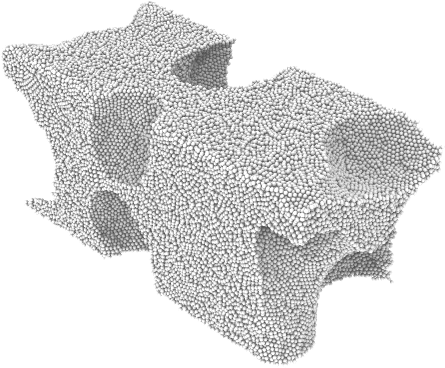
\includegraphics[width=0.40\textwidth]{./Figures/unstable}
  &
  \hspace{3mm}
  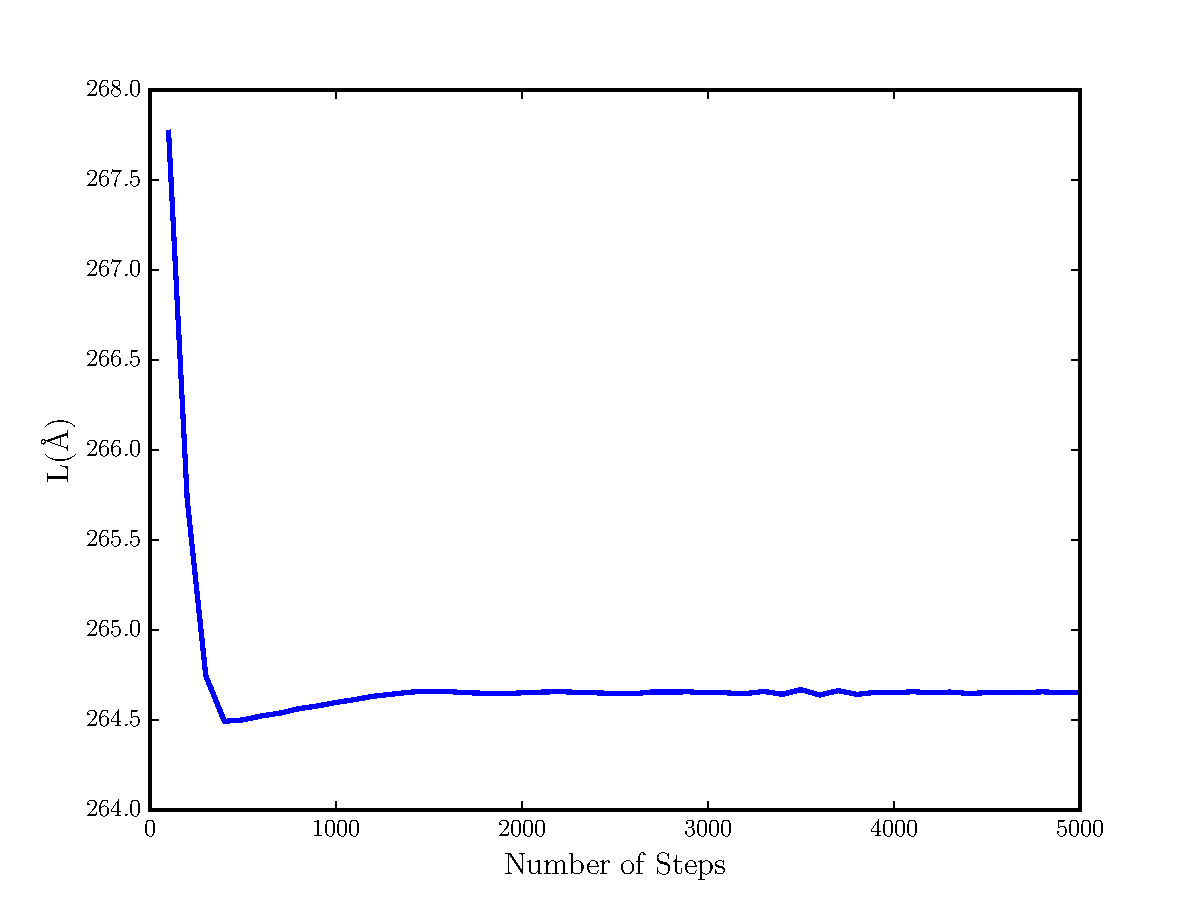
\includegraphics[width=0.50\textwidth]{./Figures/lx_npt}
  \\ (a) & (b)
  \end{tabular}
\caption{(a) A snapshot of the arrangement of atoms illustrating loss of
structural integrity of the Si bar. 
(b) Si bar length is plotted against the number of time steps during
the NPT ensemble stage of the simulation.}
\label{fig:dgsm1}
\end{center}
\end{figure}

\clearpage

%%%%%%%%%%%%%%%%%%%%%%%%%%%%%%%%%%%%%%%%%%%%%%%%%%%%%%%%%%%%%%%%%%%%%%%%%

\begin{figure}[p]
 \begin{center}
  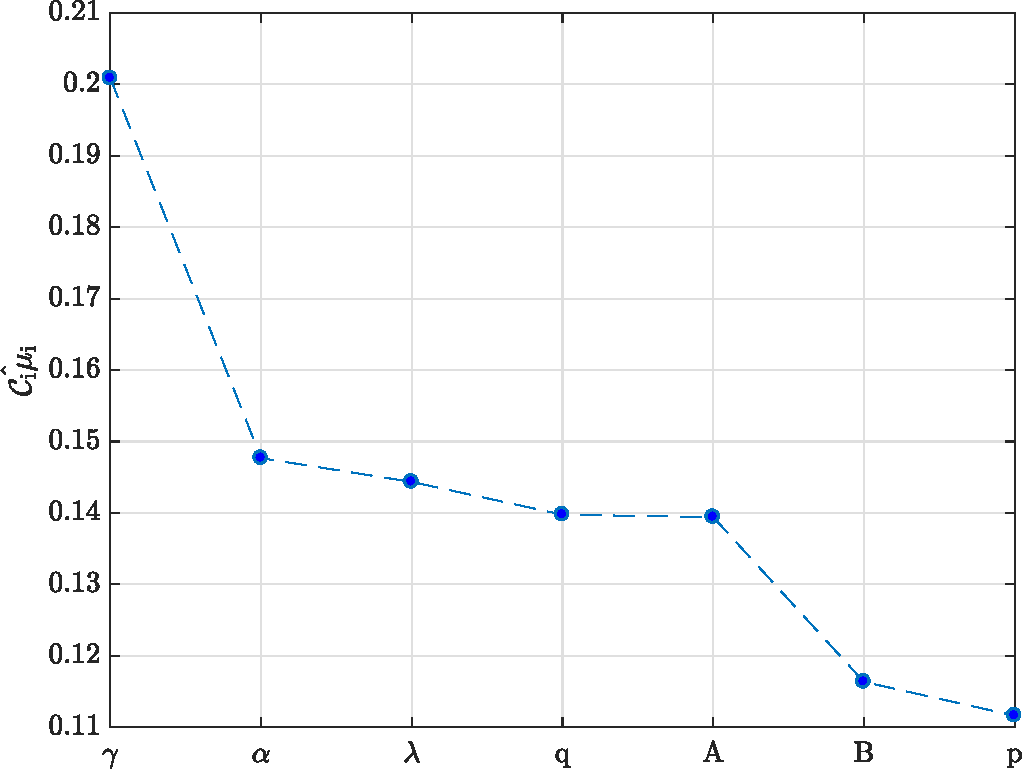
\includegraphics[width=0.70\textwidth]{./Figures/ub}
\caption{The quantity $\hat{\mathcal{C}_i\mu_i}$ as computed after 4 iterations and data at 25(7+1)
points is plotted for each SW potential parameter.}
\label{fig:ub}
\end{center}
\end{figure}

\clearpage


%%%%%%%%%%%%%%%%%%%%%%%%%%%%%%%%%%%%%%%%%%%%%%%%%%%%%%%%%%%%%%%%%%%%%%%%%

\begin{figure}[p]
 \begin{center}
  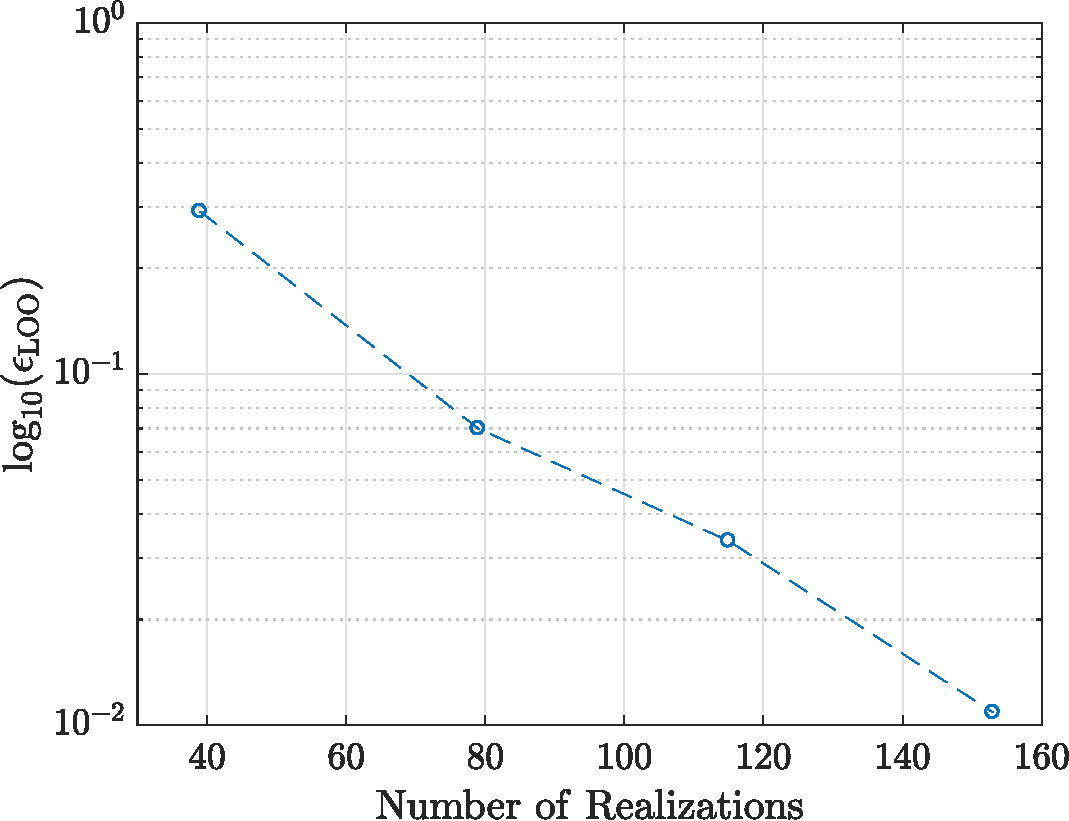
\includegraphics[width=0.70\textwidth]{./Figures/PCE5D_eloo}
\caption{A convergence study for the 5D PCE wherein the leave-one-out
error, $\epsilon_{\tiny{\mbox{LOO}}}$ is plotted against the number of
realizations or NEMD runs used to estimate the PC coefficients.}
\label{fig:loo}
\end{center}
\end{figure}

\clearpage

%%%%%%%%%%%%%%%%%%%%%%%%%%%%%%%%%%%%%%%%%%%%%%%%%%%%%%%%%%%%%%%%%%%%%%%%%

\begin{figure}[p]
 \begin{center}
  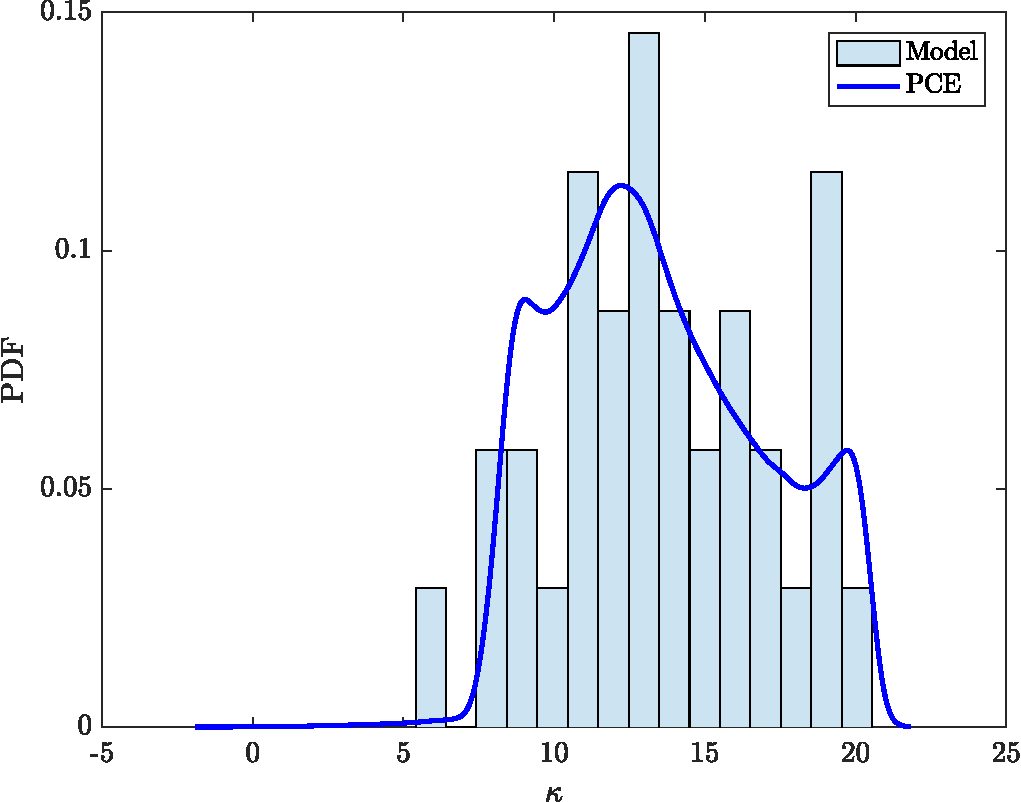
\includegraphics[width=0.70\textwidth]{./Figures/PCE5D_kde}
\caption{Comparison of bulk thermal conductivity ($\kappa$) distribution of Si based on a histogram plot
using NEMD predictions (Model) at 25 points in the 7D parameter space and a probability distribution obtained 
using kernel density estimation of  reduced order surrogate estimates of $\kappa$ for 10$^6$ samples in the 5D
parameter space.}
\label{fig:verify}
\end{center}
\end{figure}

\clearpage

%%%%%%%%%%%%%%%%%%%%%%%%%%%%%%%%%%%%%%%%%%%%%%%%%%%%%%%%%%%%%%%%%%%%%%%%%

\begin{figure}[p]
 \begin{center}
  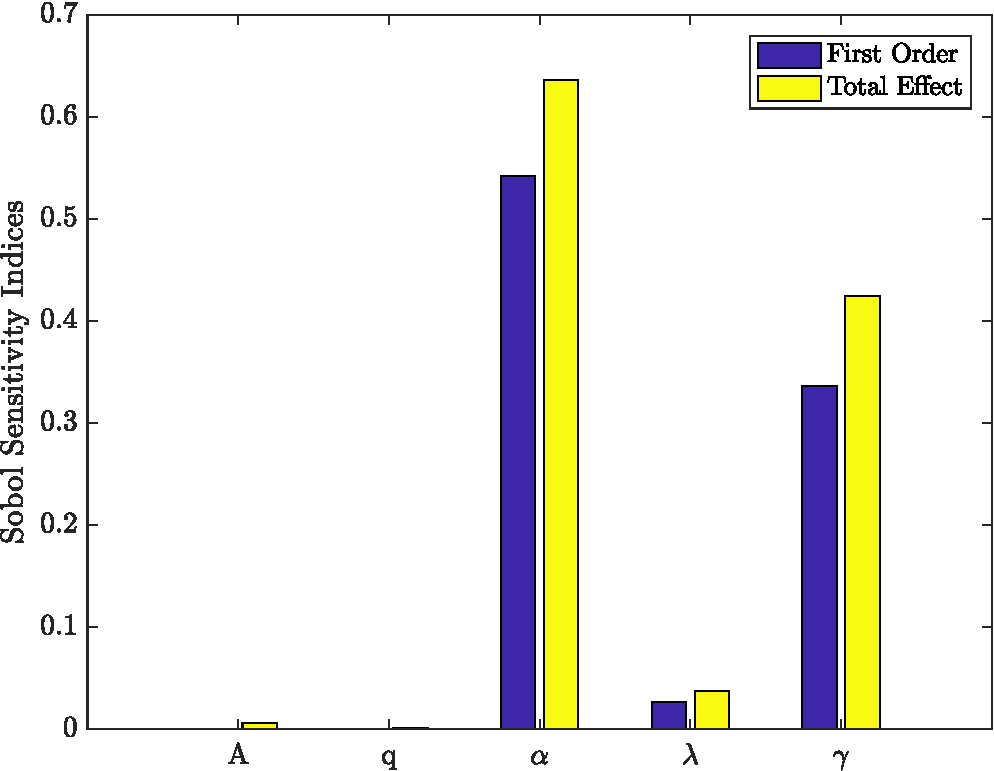
\includegraphics[width=0.70\textwidth]{./Figures/PCE5D_gsa}
\caption{Sobol first-order and total effect sensitivity indices as obtained using the reduced order PC
surrogate and 10$^{6}$ samples in the 5D parameter space. }
\label{fig:gsa}
\end{center}
\end{figure}

\clearpage

%%%%%%%%%%%%%%%%%%%%%%%%%%%%%%%%%%%%%%%%%%%%%%%%%%%%%%%%%%%%%%%%%%%%%%%%%

\begin{figure}[p]
 \begin{center}
  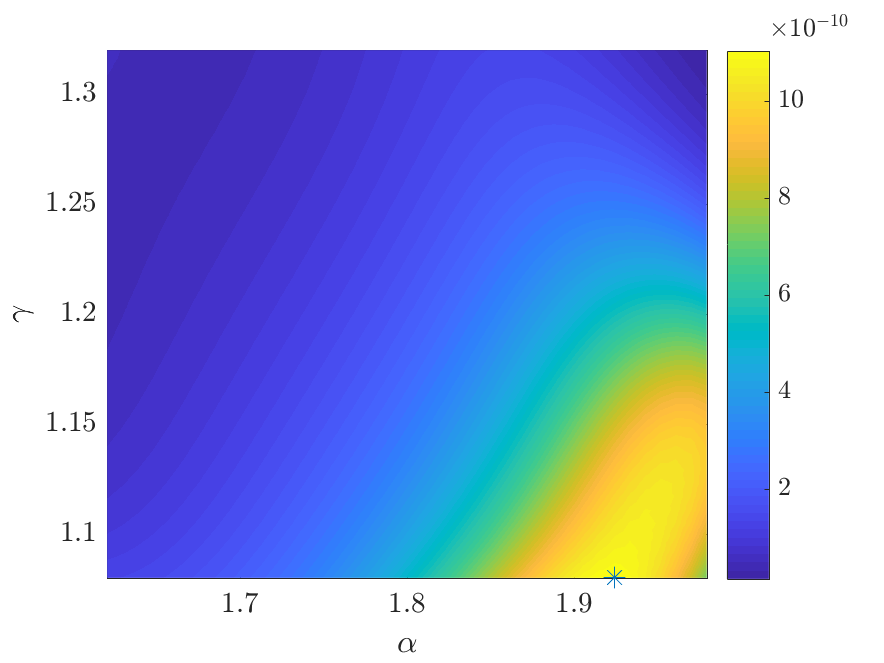
\includegraphics[width=0.70\textwidth]{./Figures/gl}
  \\ (a)
  \begin{tabular}{cc}
  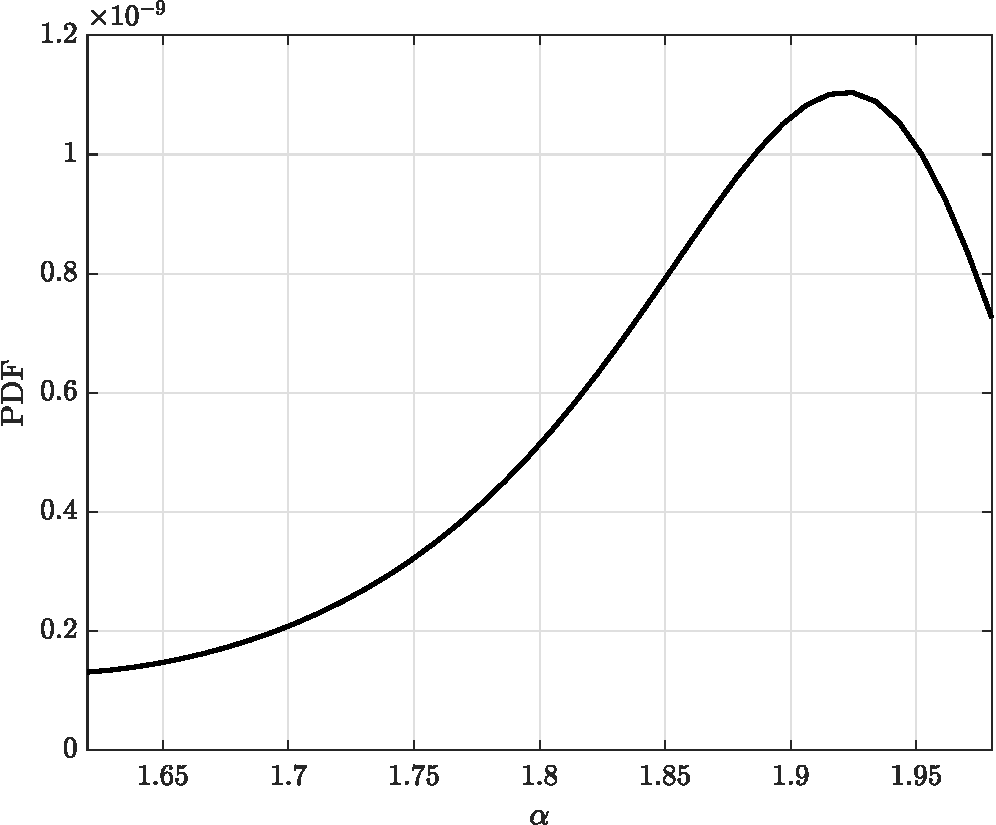
\includegraphics[width=0.50\textwidth]{./Figures/pdf_alpha}
  &
  %\hspace{3mm}
  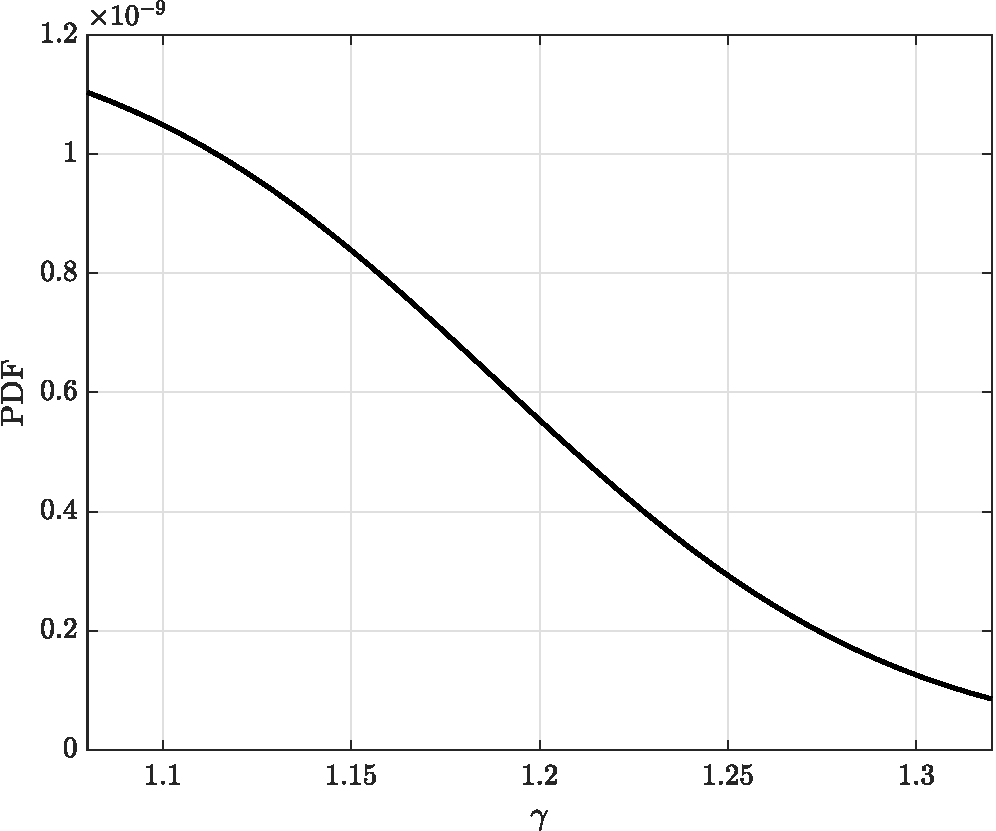
\includegraphics[width=0.50\textwidth]{./Figures/pdf_gamma}
  \\ (b) & (c)
  \end{tabular}
\caption{(a) A joint likelihood as estimated using Eq.~\ref{eq:like} is plotted on a 2D cartesian grid
 ($\alpha\times\gamma$). Point corresponding to the maximum likelihood (MLE) is also highlighted.
 The likelihood is plotted along a line passing through MLE and parallel to the $\alpha$-axis
 in (b), and $\gamma$-axis in (c).}
\label{fig:like}
\end{center}
\end{figure}

\clearpage




%%%%%%%%%%%%%%%%%%%%%%%%%%%%%%%%%%%%%%%%%%%%%%%%%%%%%%%%%%%%%%%%%%%%%%%%%


